% =============================================================================
% SECTION 5 — ANALYSIS
% Behavioural and failure-mode analysis of the 14B + r2e-gym pipeline on
% SWE-Bench-Verified. All trajectory-level statistics in this section are
% computed by parsing trajectory logs from three independent evaluation runs
% of each checkpoint (baseline = r2e-gym post-training only; ours =
% FIM-Midtrain + r2e-gym), and reported as means over the three runs.
% =============================================================================

\section{Analysis}
\label{sec:analysis}

The previous section established that FIM mid-training improves end-task
metrics. We now ask \emph{how} the resulting agent behaves differently and
\emph{where} along the trajectory the gains accrue. Both analyses are
performed on the 14B configuration with r2e-gym post-training, comparing the
post-training-only baseline (\emph{r2e-gym}) against our recipe
(\emph{FIM-Midtrain $+$ r2e-gym}). To reduce evaluation noise, every
trajectory-level statistic reported below is computed over \emph{three
independent evaluation runs} of each checkpoint and reported as the run-mean
on the SWE-Bench-Verified test set ($500$ instances per run); the
corresponding analysis on SWE-Bench-Lite ($300$ instances $\times\,3$ runs)
is reported in Appendix~\ref{app:behavior_lite} and shows the same trends.


% -----------------------------------------------------------------------------
% 5.1 Behavioural analysis
% -----------------------------------------------------------------------------
\subsection{Behavioural Changes in Agent Trajectories}
\label{sec:analysis:behavior}

We parse the SWE-Bench-Verified trajectory logs from three independent
evaluation runs of each checkpoint and aggregate trajectory-level statistics
in Table~\ref{tab:behavior}. Three findings stand out, all aligned with the
prediction of our motivating hypothesis (Section~\ref{sec:method:motivation})
that mid-training installs a structural prior for integrating external
returns into ongoing reasoning.

\paragraph{Recovery from negative observations is the largest single shift.}
We define a trajectory as containing a \emph{negative observation} if any
step's tool output matches one of a fixed set of error patterns
(stack traces, ``\texttt{No replacement was performed}'',
``\texttt{SyntaxError}'', shell errors, etc.; full list in
Appendix~\ref{app:algo}). Averaged over the three evaluation runs, the
fraction of such trajectories is essentially identical between the two
checkpoints ($88.8\%$ baseline, $91.8\%$ ours), so the agents are exposed to
comparable amounts of negative feedback. The recovery rate---the fraction
of error-containing trajectories that nevertheless terminate with a passing
patch---rises from $24.8\%$ to $28.8\%$ ($+4.0$~pp absolute, a $16\%$
relative increase). This metric tracks the precise capability our framing
predicts mid-training should support: continuing productively after an
external return contradicts the model's prior expectation.

\paragraph{Mid-training nearly eliminates the no-patch failure mode.}
Across the three baseline runs, an average of $3.0\%$ of failed trajectories
terminate with an empty \texttt{output\_patch}; after mid-training this
drops to $0.3\%$, a $\sim 10\times$ reduction. Combined with the
recovery-rate finding, the picture is that mid-training increases the
model's willingness to commit to \emph{an} edit even when intermediate
signals are noisy, rather than terminating without proposing a fix.

\paragraph{Mid-training trades terminate-fast for iterate-and-verify.}
Mid-training increases the mean trajectory length on solved tasks from
$15.1$ to $23.6$ steps and the mean number of \texttt{file\_editor}
\emph{edit} operations on solved tasks from $3.3$ to $7.4$
(Table~\ref{tab:behavior}). The action-type distribution shifts in the same
direction: the share of \texttt{search} actions falls from $15.3\%$ to
$11.0\%$ while the share of \texttt{execute\_bash} actions rises from
$19.5\%$ to $24.6\%$. The agent spends a smaller fraction of its budget on
passive repository lookup and a larger fraction on actively running scripts
and tests, then refining its edit. The cost is more steps---ours hits the
step cap on roughly $45\%$ of trajectories on average, versus $7\%$ for the
baseline---but the cost is paid on the unsolved tail; on the solved set the
additional steps translate into more correct patches.

% -----------------------------------------------------------------------------
% TABLE 7 — trajectory metrics
% -----------------------------------------------------------------------------
\begin{table}[h]
\centering
\caption{Trajectory-level behavioural metrics on SWE-Bench-Verified (14B,
r2e-gym pipeline), averaged over three independent evaluation runs of each
checkpoint. Steps, edits, and errors-encountered are means per task.
``Recovery rate'' is the fraction of trajectories that contain at least one
negative observation and nevertheless terminate with a passing patch.
``Empty patch'' is the fraction of \emph{failed} trajectories whose final
\texttt{output\_patch} is empty.}
\label{tab:behavior}
\small
\setlength{\tabcolsep}{4pt}
\begin{tabular}{l c c c c c c c}
\toprule
& \multicolumn{2}{c}{Steps / task}
& \multicolumn{2}{c}{Edits / task}
& \multicolumn{2}{c}{Errors enc.}
& Recovery \\
\cmidrule(lr){2-3}\cmidrule(lr){4-5}\cmidrule(lr){6-7}
Setting & solved & unsolved & solved & unsolved & solved & unsolved & rate (\%) \\
\midrule
+ r2e-gym
  & 15.1 & 22.4 & 3.3 & 5.4 & 3.5 & 5.8 & 24.8 \\
\textbf{+ FIM-Midtrain + r2e-gym}
  & \textbf{23.6} & \textbf{32.7} & \textbf{7.4} & \textbf{10.9}
  & \textbf{6.2} & \textbf{8.1} & \textbf{28.8} \\
\midrule
\multicolumn{8}{l}{\textit{Output and context summaries}} \\
\midrule
& \multicolumn{2}{c}{Empty patch (\% failed)}
& \multicolumn{2}{c}{Loc.\ correct (\% all)}
& \multicolumn{2}{c}{Ctx @ success (tok)}
& Pass (\%) \\
\cmidrule(lr){2-3}\cmidrule(lr){4-5}\cmidrule(lr){6-7}
+ r2e-gym
  & \multicolumn{2}{c}{$3.0$} & \multicolumn{2}{c}{$70.6$}
  & \multicolumn{2}{c}{$11{,}826$} & 26.2 \\
\textbf{+ FIM-Midtrain + r2e-gym}
  & \multicolumn{2}{c}{$\mathbf{0.3}$} & \multicolumn{2}{c}{$\mathbf{73.4}$}
  & \multicolumn{2}{c}{$\mathbf{16{,}397}$} & \textbf{29.2} \\
\bottomrule
\end{tabular}
\end{table}

\paragraph{A concrete contrast.}
The shift in termination behaviour is clearest on cases where the baseline
quits prematurely. On \texttt{scikit-learn-26323}, for instance, the
baseline trajectory runs for a single step in every run, immediately emits
\texttt{<finish>} with an empty edit and the wrong target file, and is
scored as a failure; on the same task our agent runs $\sim\!41$ steps,
applies on the order of $20$ \texttt{str\_replace} operations, observes
multiple negative tool returns, and recovers to a passing patch. Pooling
across the three runs, on the order of $\sim\!16$ of the $\sim\!55$ tasks
that ours uniquely solves on Verified have this signature: the baseline
emits \texttt{<finish>} with zero file overlap with the gold patch (often
before any negative observation has even arrived), while ours iterates past
intermediate signals and converges on a correct edit. Mid-training does not
enable a categorically new capability on these instances; it changes the
agent's stopping policy.


% -----------------------------------------------------------------------------
% 5.2 Failure mode analysis
% -----------------------------------------------------------------------------
\subsection{Where Does Mid-Training Help Most?}
\label{sec:analysis:failure}

We label every failed trajectory using a deterministic patch-quality
cascade: \emph{no-patch} (output diff is empty); \emph{localisation error}
(non-empty patch but zero file overlap with the gold patch); \emph{patch
error} (file overlap with gold patch but tests fail). We additionally
record two orthogonal behavioural flags---\emph{step-limit} (exit reason
indicates a step or token cap) and \emph{loop-like} (consecutive duplicate
actions cover at least $30\%$ of the trajectory). The labels are computed
on each of the three evaluation runs and averaged. Across the runs,
mid-training cuts no-patch failures by an order of magnitude
($\sim\!11 \to \sim\!1$ trajectories per run), trims localisation errors
slightly ($\sim\!131 \to \sim\!126$), and leaves the patch-error count
essentially flat ($\sim\!227 \to \sim\!227$); the $+15$-task gain in solved
count is therefore not explained by a single failure mode collapsing but by
a broad redistribution. The structured part of the gain becomes visible only
once we stratify by gold-patch shape.

% -----------------------------------------------------------------------------
% FIGURE 8 — pass rate by gold-patch shape
% -----------------------------------------------------------------------------
\begin{figure}[h]
\centering
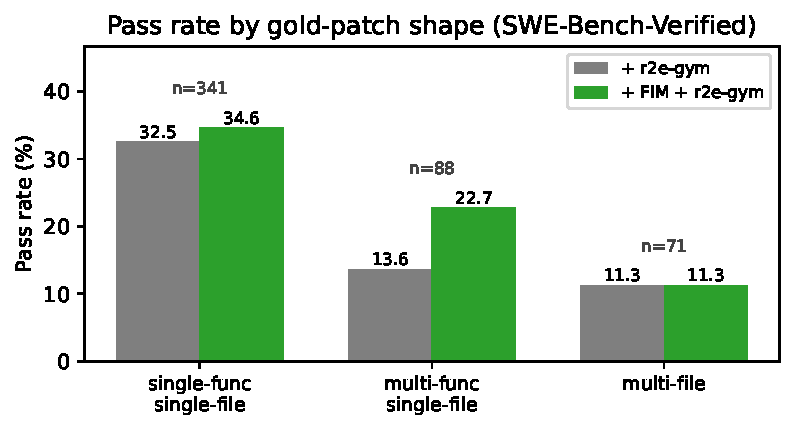
\includegraphics[width=0.62\linewidth]{figs/passrate_by_patchshape_verified.pdf}
\caption{Pass rate on SWE-Bench-Verified stratified by gold-patch shape,
averaged over three evaluation runs per checkpoint. The largest absolute
gain from mid-training is on \emph{multi-function single-file} tasks
($+9.1$~pp), followed by single-function tasks ($+2.1$~pp); multi-file tasks
remain hard for both checkpoints ($\sim\!11.3\%$ each).}
\label{fig:failure}
\end{figure}

\paragraph{The gain concentrates on multi-function reasoning.}
Stratifying the $500$ Verified tasks by the shape of the gold patch
(Figure~\ref{fig:failure}) reveals a structured concentration of gain. Among the $88$ tasks whose gold patch modifies $\ge 2$ functions
within a single file, the baseline solves $13.6\%$ on average and ours
solves $22.7\%$, an absolute gain of $+9.1$~pp---more than $4\times$ the
gain on the $341$ single-function tasks ($+2.1$~pp). Per-instance
head-to-head on this bucket (taking, for each task, the run-majority outcome
of each checkpoint) shows ours uniquely solves about twice as many tasks as
the baseline does; the same per-instance comparison on the single-function
bucket has ours ahead by roughly $1.2\times$. This is the slice most
directly aligned with the function-graph structure exposed by mid-training:
tasks where the agent must follow control- and data-dependencies between
sibling and caller-callee functions inside a file before producing a
coherent edit. We read this as a closing-loop confirmation of the
isomorphism argument in Section~\ref{sec:method:motivation}: the failure
modes that recede are the ones whose successful resolution requires
reasoning about how a callee's return interacts with downstream code in the
same module.

\paragraph{Multi-file tasks are not differentially helped.}
On the $71$ Verified tasks whose gold patch spans $\ge 2$ files, both
checkpoints solve $\sim\!11.3\%$ on average; per-instance head-to-head on
this bucket is balanced. We attribute this to a mismatch in granularity:
our function-aware FIM mid-training operates at the function level within
files, so cross-file coordination is not directly trained for. Extending the
selection algorithm to cross-file function pairs is a natural follow-up.

\paragraph{Why the no-patch mode collapses.}
The baseline no-patch failures recovered by mid-training are distributed
across all task buckets and are not concentrated in any single repository.
In every recovered case the baseline emitted \texttt{<finish>} without
applying any \texttt{str\_replace}, while ours applied at least one edit.
We interpret this as a direct consequence of the fill-in-the-middle training
signal: under FIM the model is always conditioned to produce a non-empty
token span between the prefix and suffix, and we observe that this
disposition survives the post-training pipeline.


% -----------------------------------------------------------------------------
% 5.3 General capability forgetting check
% -----------------------------------------------------------------------------
\subsection{Preservation of General Capabilities}
\label{sec:analysis:forgetting}

% NOTE [author]: this subsection is a placeholder. The trajectory-level
% analysis above does not require additional benchmarks, but the scaffold
% reserves space for an MMLU / MATH / IFEval forgetting check on the 14B
% checkpoints. The numbers are not yet measured. Decide before submission
% whether to (i) run the three benchmarks and report a 3-row table here,
% (ii) move this paragraph into the appendix, or (iii) cut the subsection.
% Suggested framing if kept (one paragraph, no table):
%   "Section~\ref{sec:exp:gen} already shows that mid-training narrows the
%    capability regression that r2e-gym post-training induces on non-agent
%    coding benchmarks. To check whether the same holds for non-coding
%    general-capability benchmarks, we evaluate the 14B checkpoints on
%    MMLU, MATH and IFEval; results in Appendix~\ref{app:results}."
\textcolor{red}{[TBD: forgetting check on MMLU / MATH / IFEval at 14B,
or move to Appendix~\ref{app:results}, or cut. See author note in source.]}
